\chapter{Clustering Interface Design}

% Clustering introduction, what is it, how does it work?
% Clustering nodes with mouse
% Cluserting with regex
% Useful naming of nodes
% Avoiding false dependencies

Clustering in this paper is the action of taking a set of nodes removing them from the graph and replacing them with a single composite node. An example of this is in Figure~\ref{fig:clustering-example} where you can see the node \textit{Fitness-Summary} and all its children have been clustered to create the composite node named `Fitness Data'. There is two primary ways of creating clusters, the first is automatically based on properties of the nodes or other heuristics, the second is via manual selection by the user. Previous research has been done into automatic clustering~\cite{Borkin2013,Seltzer2011}, what we focus on in this thesis is expanding on the work done in manual clustering~\cite{Biton2007} by designing an interface that allows effective clustering not just as a method of graph simplification, but as a way of conveying information.

The primary requirements for manual clustering where that it be simple to use and intuitive to new users. It should be easy for users to cluster nodes together without been shown how to. But it must also be powerful for expert users, so that someone who deals with provenance on a daily basis can quickly and easily create summary graphs with composite nodes in a minimal amount of time and effort.

\begin{figure}[h]
  \centering
  \begin{subfigure}[t]{0.5\textwidth}
    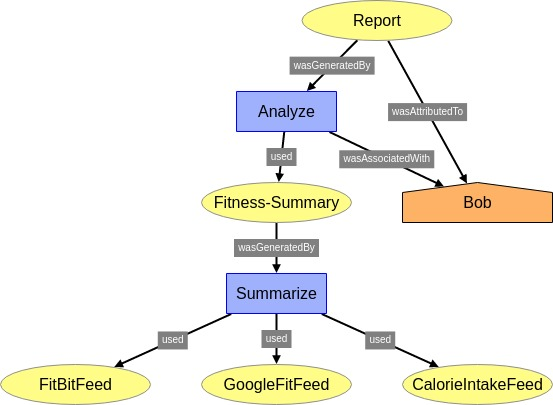
\includegraphics[width=0.9\textwidth]{clustering-example-2}
    \caption{The full provenance graph with no clustering.}
  \end{subfigure}
  ~
  \begin{subfigure}[t]{0.5\textwidth}
    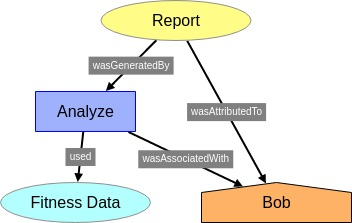
\includegraphics[width=0.9\textwidth]{clustering-example-1}
	\caption{The node \texttt{Fitness-Summary} and all its children have been grouped into a composite node \texttt{Fitness Data}}
  \end{subfigure}
  \caption{Above is a provenance graph showing the lineage of a report on Bob's fitness. On the left is the full graph, on the right a cluster has been manually created.}
  \label{fig:clustering-example}
\end{figure}

To fulfil these requirements I designed two different mechanisms for clustering, one for novice users and one for expert users. Although both can be used by either category of user it is easiest to differentiate them this way. 

\section{Manually clustering nodes}
\label{sec:user_defined_clusters}

The first method I designed was for novice users and works the following way: a user selects multiple nodes by clicking on them whilt holding down \textit{ctrl}, each selected node is outlined red as an indicater to the user that they are selected. Users can then cluster the nodes together by selecting a group function from a list of contextual actions. 

This allows users to cluster nodes together with little to no prompting from an expert. However it has the drawbacks of only been viable to a small number of nodes as selecting more than a dozen or so nodes is tedious and error prone. 

In order to allow precise and powerful node selection I designed a second way of allowing users to cluster nodes via a regex search function. Using the search bar users can input regex strings and matching nodes will be selected (same as manually clicking, selected nodes are outlined red). Once the user had tweaked the query to their liking they can group the nodes using the same technique as before; selecting the group function from a list of contextual actions. To make it easier to create multiple clusters quickly, pressing \textit{enter} while in the search field will cluster together the currently selected nodes, this allows users to quickly create a series of clusters without having to move their hands from the keyboard (a detailed analysis of the effectiveness of this can be found below in Section~\ref{sub:goms_analysis}). The regex query currently searches all properties and attributes of nodes, a future path of work would be to expand it so that you can match on specific properties.

Creating these two methods of clustering allows users to easily be introduced to the concept of clustering in an intuitive way, by clicking on nodes, then expand to the more complex and powerful tool of regex searching. Details on how these two methods where implemented can be found in Section~\ref{sec:clustering}.

\subsection{GOMS analysis}
\label{sub:goms_analysis}

GOMS is a method of predicting how long a task will take. It is outlined in \citetitle{card1983psychology} by \citeauthor{card1983psychology}~\cite{card1983psychology}. It can be used to compare how long it takes to accomplish a tasks in different ways. In this case I use it to compare the speed difference between \textit{ctrl+click} clustering and search clustering.

A task is given a series of letters to represent what happens when a user tries to accomplish that task. For example, using the \textit{ctrl+click} method to select the nodes as shown in Figure~\ref{fig:clustering-example} would be: HMPCR HK MPCR MPCR MPCR MPCR MPCR. Each letter represents something that occurs:

\begin{itemize}
\item K - keypress
\item P - point with mouse
\item C - click with mouse
\item H - home hands on new device
\item M - mentally prepare
\item R(t) - system response time
\end{itemize}

So using this we can break down the GOMS string for \textit{ctrl+click} as meaning the follwing:

\begin{itemize}
	\item HMPCR - User moves hand to mouse and points and clicks at \texttt{Fitness-Summary} node (node is hilighted with red outline)
\item HK - User moves hand to keyboard and holds down \textit{ctrl} button
\item MPCR - User moves mouse and clicks the \textit{Summarise} node.
\item MPCR - User moves mouse and clicks the \textit{FitBitFeed} node.
\item MPCR - User moves mouse and clicks the \textit{GoogleFitFeed} node.
\item MPCR - User moves mouse and clicks the \textit{CalorieIntakeFeed} node.
\item RMKPCR - User sees group link in contextual actions, stops hodling down \textit{ctrl}, moves mouse to the group link and clicks it. The nodes move together and create a composite node.
\end{itemize}

Similarly, search clustering can be represented as the follwing: 

\begin{itemize}
\item HMC - User moves hand to mouse and selects the search button from the toolbar
\item RMPC - The search panel is show. The user moves the pointer and clicks the text input field of the search panel.
\item HMKKKKKKKKKKKKKK - User moves hands to the keyboard and types the following regex ``Summzarize|Feed''
\item KR - User presses \textit{enter}, the nodes move together and create a composite node.
\end{itemize}

We can then assign time values to each of these tasks as seen in Table~\ref{tab:goms-times}. The times used here are based on those published in the \citetitle{card1983psychology} book~\cite{card1983psychology}. Note that these times assume an expert (familiar with the domain and application), error free user.

\begin{table}[h]
	\centering
		\def\arraystretch{1.5}
	\caption{A list of GOMS tasks and their assosiated timing.}
	\label{tab:goms-times}
	\begin{tabular}{| c | l | c |}
		\hline
		\textbf{Letter} & \textbf{Desc.} & \textbf{Time (seconds)} \\
		\hline
		\hline
		K & keypress & .08 - 1.20 \\
		P & point with mouse & .8 - 1.5 (Fitt's Law) \\
		C & click with mouse & .2 \\
		H & home hands on new device & .4 \\
		M & mentally prepare & 1.35 \\
		R(t) & system response time & 0 \\
		\hline
	\end{tabular}
\end{table}

\begin{table}[h]
	\centering
		\def\arraystretch{1.5}
	\caption{The resulting times from GOMS analysis of the two methods for clustering a set of nodes, \textit{ctrl+clicking} and search clustering. I assume that it takes about 1.2 seconds for the user to point with the mouse, and that they're a moderately fast typer taking 0.2 seconds per keypress.}
	\label{tab:goms-results}
	\begin{tabular}{| l | l | c |}
		\hline
		\textbf{Method} & \textbf{GOMS string} & \textbf{Time (seconds)} \\
		\hline
		\hline
		Ctrl+click & HK MPCR MPCR MPCR MPCR RMKPCR & 14.54 \\
		Search group & HMC RMPC HMKKKKKKKKKKKKKK KR & 9.44 \\
		\hline
	\end{tabular}
\end{table}

As seen in Table~\ref{tab:goms-results} it takes approximately 15 seconds to conduct the grouping of \texttt{Fitness-Summary} and its children using the \textit{ctrl-click} method, while only taking 10 seconds when using the search group method. These results would vary depending on how fast a typer the user was and how good their fine motor skills where. It also depends on how ``searchable'' the nodes you wish to group are, in cases where the nodes have no common property values it may be faster to select the nodes using the \textit{ctrl-click} method. However in any case where the nodes you want to select share a property with the same value, the search group method is likely to come out on top because multiple nodes can be selected with a single string compared to having the limit of one node been selected by one click.

\section{Challenges}
\label{sec:naming_composite_nodes}

The main challenge in clustering nodes is that of naming. Once a composite node is created it must be given a name. In an early version of the ProvOwl system nodes where given short random alpha-numeric names. We found that this soon made the graph incomprehensible and relied on the user manually renaming each node (described in Section~\ref{sec:details_on_demand}) in order for the graph to be usable. 

Ideally an interface would give clusters a name describing its contents. I found this is a much harder problem than it at first seems and requires domain level knowledge as well as models of the user and what information is important to them. For example, the nodes \texttt{sunflower}, \texttt{daffodil} and \texttt{poppy} where to be clustered. Naively it would be useful to name the cluster \textit{plants}, however if the user was a florist this may be too broad a definition and the label \textit{flowers} would be more appropriate.

In some fields this problem has been solved by limiting the number of unknown things. For example, if you create a folder of apps on an iPhone it is automatically named with a label appropriate to the applications inside of it. A folder full of photography apps may be labelled \textit{Photography}. However this differs from the problem we are solving in a variety of ways. Firstly the number of possible labels is limited to the categories in the Apple app store, this creates a finite set of possible label options. Secondly, when an application is uploaded to the app store the author publishes metadata with it such as the category of the app. Using this metadata makes it much easier to name clustered items. Having the same level of metadata in provenance files could be accomplished by having tags associated with each node, these tags could then be used to effectively name a cluster simply by selecting the most used tag from the group of nodes to be clustered. However there is currently no tagging system for provenance nodes.

Our currently, still simple approach uses the name of the node in the cluster closest to the root with the text ``group'' appended to the end. While this doesn't always create the most effective names for clusters, it gives the user a point of reference when looking at clusters which in most cases is enough to trigger the user to what the contents of the cluster is. During usability studying users never renamed nodes unless they specifically wanted to convey information to another user.

\begin{figure}[h]
	\centering
	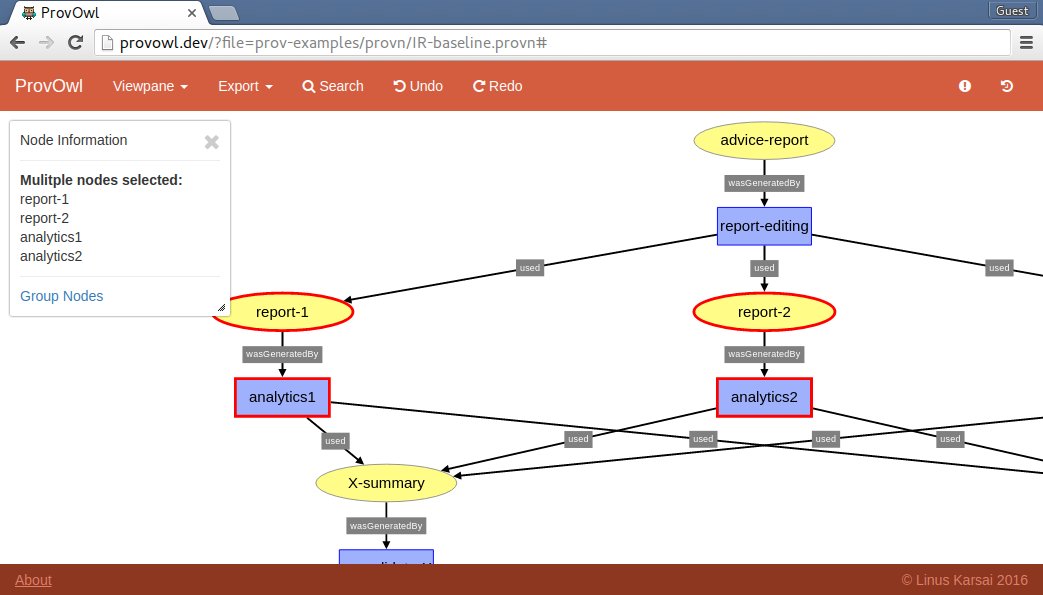
\includegraphics[width=\linewidth]{naming1}
	\caption{Using the \textit{IR-baseline} example the user has selected four nodes for grouping, essentially those related to \texttt{report-1} and \texttt{report-2}.}
	\label{fig:naming1}
\end{figure}
\begin{figure}[h]
	\centering
	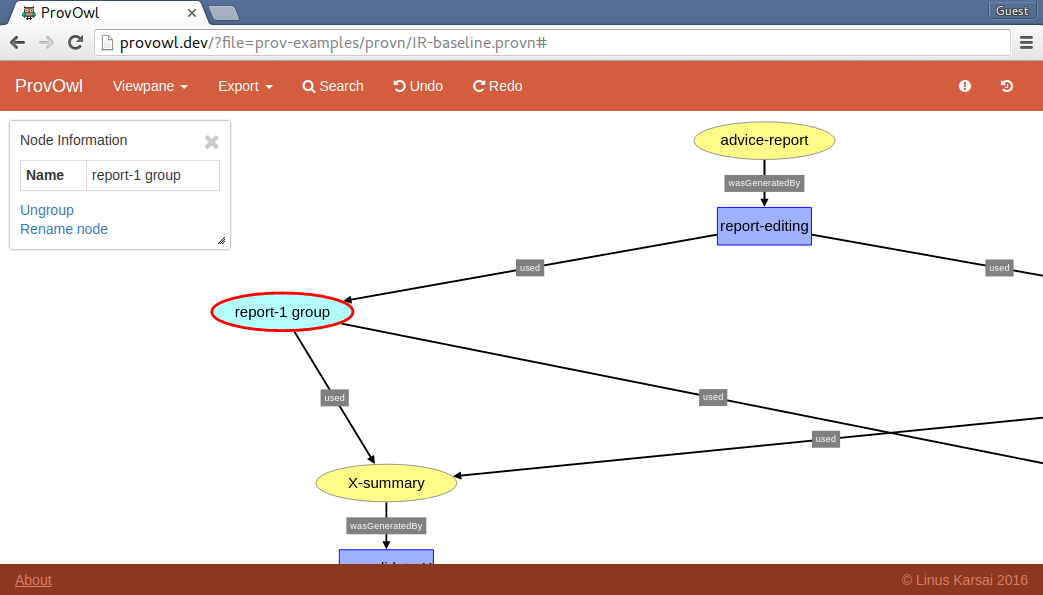
\includegraphics[width=\linewidth]{naming2}
	\caption{When clusterint the four nodes selected in Figure~\ref{fig:naming1} ProvOwl creates a composite node using the name of the node closest to the root (in this case breaking a tie by alphabetical order).}
	\label{fig:naming2}
\end{figure}
\clearpage

